% Template for Affective Computing and Intelligent Interaction (ACII)
%
% Modified 2022-03-15 : Desmond Ong (desmond.c.ong@gmail.com)     
%.      -- update for ACII2022, added section for Ethical Impact Statement
%

\documentclass[conference]{IEEEtran}
\IEEEoverridecommandlockouts
% The preceding line is only needed to identify funding in the first footnote. If that is unneeded, please comment it out.
\usepackage{cite} \usepackage{amsmath,amssymb,amsfonts}
\usepackage{algorithmic} \usepackage{graphicx} \usepackage{textcomp}
\usepackage{xcolor} \usepackage{hyperref} \usepackage[normalem]{ulem}

\def\BibTeX{{\rm B\kern-.05em{\sc i\kern-.025em b}\kern-.08em
    T\kern-.1667em\lower.7ex\hbox{E}\kern-.125emX}}
\begin{document}

\title{Emotion Twenty Questions Dialog System for
  Lexical Emotional Intelligence \thanks{We thank the following for
    support and funding: University of St. Thomas Center for Applied
    Artificial Intelligence and University of St. Thomas Center for
    Faculty Development Graduate Research Team Grant.}  }

\author{\IEEEauthorblockN{Abe Kazemzadeh}
\IEEEauthorblockA{\textit{Graduate Programs in Software} \\
\textit{University of St. Thomas}\\
St. Paul, MN, U.S.A. \\
%abe.kazemzadeh@stthomas.edu,
orcid:0000-0002-1851-294X}
\and
\IEEEauthorblockN{2\textsuperscript{nd} Given Name Surname}
\IEEEauthorblockA{\textit{dept. name of organization (of Aff.)} \\
\textit{name of organization (of Aff.)}\\
City, Country \\
email address or ORCID}
\and
\IEEEauthorblockN{3\textsuperscript{rd} Given Name Surname}
\IEEEauthorblockA{\textit{dept. name of organization (of Aff.)} \\
\textit{name of organization (of Aff.)}\\
City, Country \\
email address or ORCID}
\and
\IEEEauthorblockN{4\textsuperscript{th} Given Name Surname}
\IEEEauthorblockA{\textit{dept. name of organization (of Aff.)} \\
\textit{name of organization (of Aff.)}\\
City, Country \\
email address or ORCID}
\and
\IEEEauthorblockN{5\textsuperscript{th} Given Name Surname}
\IEEEauthorblockA{\textit{dept. name of organization (of Aff.)} \\
\textit{name of organization (of Aff.)}\\
City, Country \\
email address or ORCID}
\and
\IEEEauthorblockN{6\textsuperscript{th} Given Name Surname}
\IEEEauthorblockA{\textit{dept. name of organization (of Aff.)} \\
\textit{name of organization (of Aff.)}\\
City, Country \\
email address or ORCID}
}

\maketitle

\begin{abstract}
  %A brief background introduction and description of the system:
  
  This paper presents a web-based demonstration of Emotion Twenty
  Questions (EMO20Q), a dialog game whose purpose is to study how
  people describe emotions.  EMO20Q can also be used to develop
  artificially intelligent
  % or artificial intelligent 
  dialog agents that can play the game.  In
  previous work, an EMO20Q agent used a sequential Bayesian machine
  learning model and could play the role of asking questions.  Newer
  transformer-based neural machine learning models have made it
  possible to develop an agent for the question-answering role.

  %a summary of the technical contributions of the system:

  This demo paper describes the recent developments in the
  question-answering role of the EMO20Q game, which requires the agent
  to respond to more open-ended inputs.  Furthermore, we also describe
  the design of the system, including the web-based front-end, agent
  architecture and programming, and updates to earlier software used.

  %results of a formal evaluation or experiment to be conducted during
  %the demo, if applicable:

  The demo system will be available to collect pilot data during
  the ACII conference at and this data will be used to inform future
  experiments and system design.

  % Our early results indicate that ...

  %a url to a video recording or screenshots of how the system works:
    %what would be a good url for emo20q?  emo20q.org? emo20q.ai?

  An example of the demo system can be seen in
  Fig.~\ref{fig:emo20q-flask-websocket} and the live system can be
  accessed at \href{https://emo20q.org}{emo20q.org}.
\end{abstract}

\begin{IEEEkeywords}
emotions, natural language processing, dialog, question-answering, EMO20Q
\end{IEEEkeywords}

\begin{figure}[h]
\centering
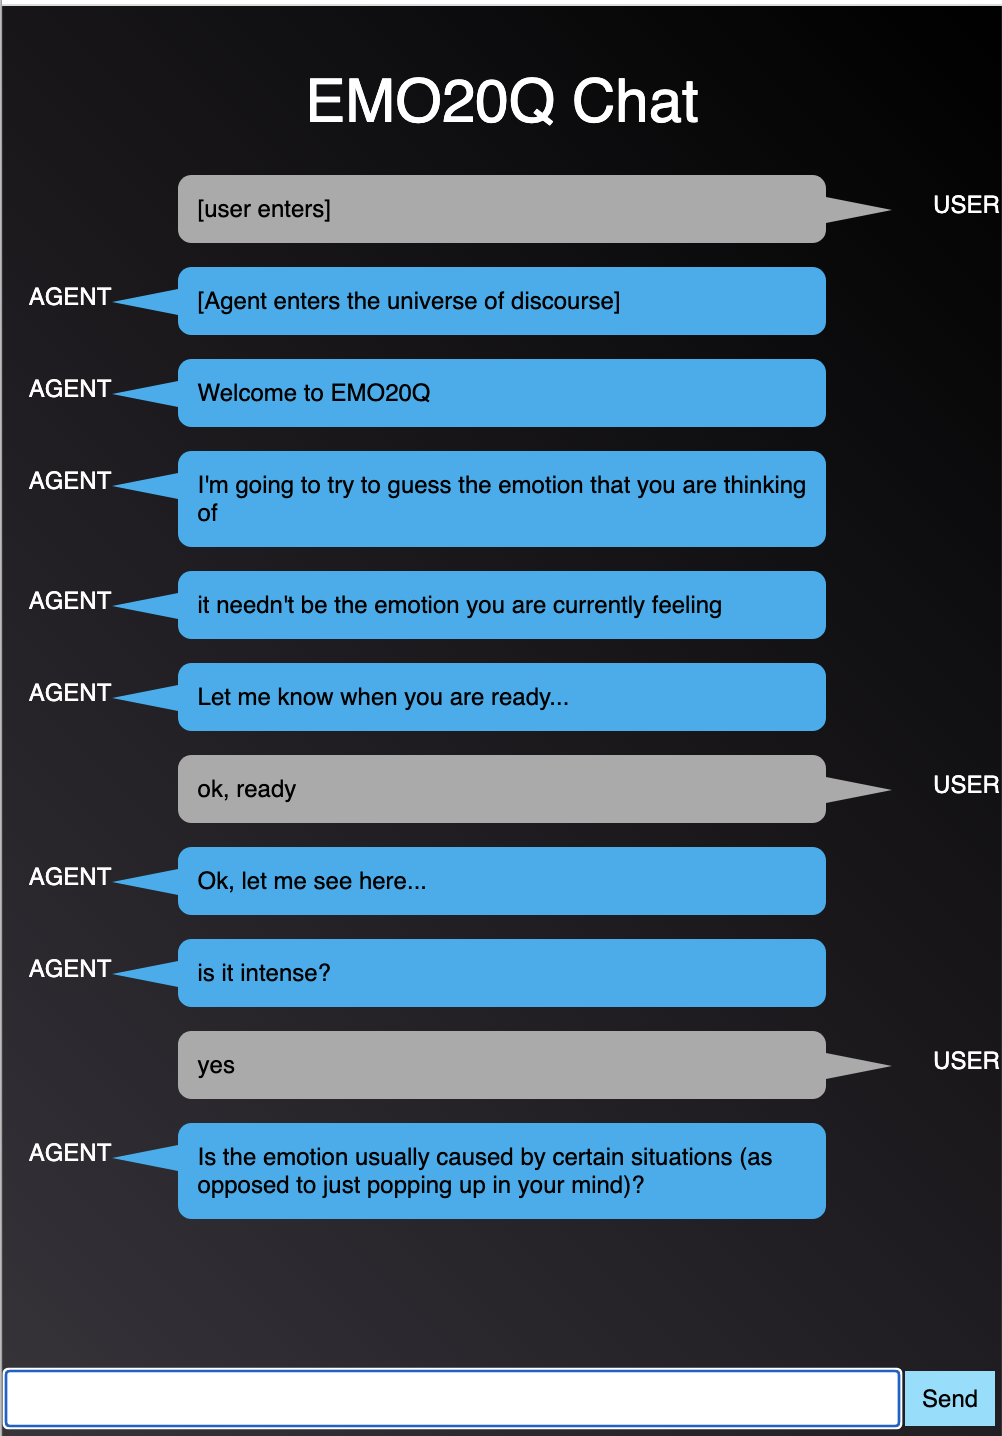
\includegraphics[width=0.5\textwidth]{emo20q-flask-websocket}
\caption{Example of the web-based front end to the EMO20Q dialog
  system.}
\label{fig:emo20q-flask-websocket}
\end{figure}


\section{Introduction}

This demo system aims to use a dialog agent to collect question-answer
data about human emotions.  We use the emotion twenty questions game
(EMO20Q) as the experimental setting.  In EMO20Q, one player picks an
emotion word and the other player tries to guess it in twenty or fewer
turns. The player that picks the emotion word is the {\it answerer},
because they answer questions about the emotion word that they picked.
The player who tries to guess the emotion word is the {\it questioner}
because they ask questions in order to identify the emotion word.

Both player roles for EMO20Q could be played by humans or computers.
Our past approach involved having humans play EMO20Q and using this
data to train artificially intelligent dialog agents to play the
questioner role \cite{Kazemzadeh2012}.  This work used a sequential
Bayesian probablistic model for the questioner role in the game
\cite{Kazemzadeh2012}: the input was a sequence of question-answer
pairs. The question set comes from human-human dialogs and the
particular question that the agent asks is chosen based on the dialog
history. The answers come from the user's corresponding responses.
Posterior probabilities of the emotion words are updated based on
these sequential question-answer inputs.

At the time of our earlier
work, we considered the questioner role to be easer because the set of
questions was predetermined based on the human-human dialogs, so the
only open-ended input is the answers to yes-no questions.  These are
not restricted to yes or no, but it is trivial to bucket these
responses into yes/no/other categories.

Our current work aims to extend the approach to a dialog agent that
can play the answerer role. In this case, the agent picks the emotion
word from previously seen words (todo: include how many emotion words)
and answers questions posed by the user. In this case, the agent's
input is much more open-ended: any possible yes/no question about
emotions.  Many questions, especially earlier in the game, have been
seen before (e.g., ``is it a positive emotion?'', ``is it a negative
emotion?'', ``is it an emotion that is directed at another person?'',
``is it an emotion that lasts along time?''), but in principle, any
question could be asked.  To deal with this open-ended question task,
we aim to leverage neural large language models (LLM), which encode
linguistic knowledge from large pre-training data sets into neural
networks, which can then be fine-tuned into task specific models with
relatively smaller datasets.


Our goal for the current work is to use the system to continue to test
hypotheses about how well automated systems can understand language
about emotions.

The current system still involves an automated agent
playing with a human user.  However, with dialog agents that can play
both both roles, two automated agents could play EMO20Q with each
other.




%% \section{Stash}
%% \begin{itemize}
%% \item \href{https://acii-conf.net/2022/calls/call-for-demos-2/}{call for demos}
%% \item \href{https://acii-conf.net/2022/authors/submission-guidelines/}{submission guidelines}
%% \item submit using
%%   \href{https://easychair.org/conferences/?conf=aciioo2022}{EasyChair}
%% \end{itemize}

\section{Web Front End}

To simply display the front end of the demo system we used Flask, a
lightweight Python web framework.  Using the simple request-response
interaction of a basic web server would have been an option, but it
would require a page reload for every dialog turn and could result in
slow response times, especially in cases where prediction requires
beam search (the question answering role).  To prevent page reloads
and response delays, we used Websockets via the Socket.io library,
which enables bidirectional communication between the browswer and
web server.  Dialog events, i.e. turns from the user (via the browser)
or agent (via the server), trigger updates to a typical speech bubble
dialog display, as seen in Fig.~\ref{fig:emo20q-flask-websocket}.

\section{Dialog Agent}

The dialog agent was trained using a method inspired by wizard of Oz
approaches \cite{Fraser1991} and games with a purpose
\cite{Ahn2004}. First both roles of EMO20Q were played by non-expert
human players. Then later work created automated agent for the
question-asking role by finding the conditional probabilities of
(question, answer) pairs given emotion words and using these to create
a sequential Bayesian probabilistic model \cite{Kazemzadeh2012}.  Our
current work has focused on the question-answering role.  This current
work has benefitted from recent trends in transfer-learned deep neural
language models.  In particular
%, we used BERT, an encoder only system, and
T5 \cite{Raffel2020}, an encoder-decoder pretrained language model for
our demo system, though a more systematic examination of other models
is planned for future work.

The programming of the agent is based on a generalized pushdown
automaton (GPDA) \cite{Allauzen2012}.  The abilities of a general
finite state automata are sufficient for most of the dialog behavior,
but the pushdown stack is used to maintain contextual information that
represents short-term/working memory in the question-asking role. The
transition graph of the automaton is implemented with NetworkX Python
library.


\section{Discussion}
Should the transformer use an encoder + classifier approach, or a
encoder + decoder (sequence-to-sequence) approach?

The former (classifier) is arguably simpler and would fit better with
the existing yes/no/other approach (though binary vs. ternary). The
latter would allow more diverse, fluent type responses besides yes/no
(and perhaps other for soft/fuzzy classfications)

Django vs flask. Flask is simpler to use but lacks the standardized
user management functions (authentication/login, emails), model view
controller framework, database ORM, etc., that comes included in
Django.  While the data generated from the dialogs is json, other
features of a RDBMS system would be useful in cases where structured
data is maintained (more digested data like emotion vocabularies, user
information for demographic information and querying user history).

If we use the decoder generation as output, what should the generation
params be?  greedy, beam, etc

ordering of EMO20Q roles: will playing as answerer first prime the
human user to reuse the agent's questions?

\section{Future Work}

We intend to use this demo system to collect data and use it to test
models and hypotheses primarily for question-asking role.  Currently,
the system uses a basic question answering model by fine tuning the
pretrained T5 model.  Deep learning models have proliferated and there
are many other models and hyperparameters to test.

%Also, the game
%setting may be a possible application for adversarial training.


\section{Ethics Statement}

This research has been approved by the University of St. Thomas
institutional review board (IRB).  Data is not collected with
personally identifying information (PII) and the collected with be
examined for PII before public dissemination.



\bibliographystyle{ieeetr}
\bibliography{../../../Dropbox/org/reference/AbesBigBibliography}
\end{document}
